%%%%%%%%%%%%%%%%%%%%%%%% VRES LATEX %%%%%%%%%%%%%%%%%%%%%%%


% This sets the style of the document, you can use different built in styles, create your own .cls files or download ones from the Internet. This one is fairly standard to use
\documentclass[18pt]{article}

%%%%%%%%%%%%%%%%%%%%%%%%%%%%% Packages %%%%%%%%%%%%%%%%%%%%%%%%%%%%%%

% This package is handy for captioning figures, you can set caption style here as well
\usepackage[font={large,it}]{caption}
\usepackage[a4paper, portrait, margin=0.5in]{geometry}
% This is important for position images as latex will put your image where it best fits unless you tell it otherwise
\usepackage{float}

% If you want images this is necessary
\usepackage{graphicx}
\usepackage{subcaption}
\graphicspath{{./images}}
% You can use this to set your margin size
%\usepackage[margin=25mm]{geometry}

% Allows you to do things such as headers and footers
\usepackage{fancyhdr}

% This needs to be in here if you want to set up your document with more than one column in sections 
\usepackage{multicol}

% Here are a few packages that help with formatting equations, you may not need to use this but I find align* from amsmath particularly useful
\usepackage{amsmath,amssymb,amsthm,textcomp,amsfonts,amsthm,mathrsfs}

% Enhances Latex's cross referencing
\usepackage{cleveref}
\usepackage{hyperref}
\hypersetup{colorlinks=true}
\hypersetup{linkcolor=blue}
\usepackage{xcolor}
\usepackage{physics}
\usepackage{gensymb}
\usepackage{mathrsfs}
% Also not necessary but I find it handy when formatting arrays and matrices
\usepackage{array}
\usepackage{xfrac}

%% These packages you'll need to download a .sty file before you can use

% This allows really nice formatting for MATLAB code, it's the main plug in package that I use
\usepackage[numbered,framed]{mcode}
\usepackage{mathrsfs}
\usepackage{hyperref}
\hypersetup{colorlinks=true}
\hypersetup{linkcolor=blue}
\usepackage{xcolor}
\usepackage{physics}
\usepackage{gensymb}

%% Feel free to add any more packages you want!!!
\usepackage{indentfirst}
\usepackage{parskip} 
\setlength\parindent{0pt}
%\setlength{\parskip}{1cm plus4mm minus3mm}
\usepackage{csquotes}
\usepackage{mathtools}
\newcommand{\Lim}[1]{\raisebox{0.5ex}{\scalebox{0.8}{$\displaystyle \lim_{#1}\;$}}}

%%%%%%%%%%%%%%%%%%%%%%%%% Setup the document %%%%%%%%%%%%%%%%%%%%%%%%

\lstset{basicstyle=\scriptsize\ttfamily,breaklines=true}
\renewcommand{\thesubsection}{\thesection\alph{subsection}.}
\renewcommand{\thesubsubsection}{\indent \roman{subsubsection}}

\numberwithin{equation}{section} % Number equations within sections (i.e. 1.1, 1.2, 2.1, 2.2 instead of 1, 2, 3, 4)
\numberwithin{figure}{section} % Number figures within sections (i.e. 1.1, 1.2, 2.1, 2.2 instead of 1, 2, 3, 4)
\numberwithin{table}{section} % Number tables within sections (i.e. 1.1, 1.2, 2.1, 2.2 instead of 1, 2, 3, 4)

\newcommand{\horrule}[1]{\rule{\linewidth}{#1}} % Create horizontal rule command with 1 argument of height

\title{	
	\normalfont \normalsize 
	\textsc{Queensland University of Technology, Vacation Research Experience Scheme} \\ [25pt] 
	\horrule{0.5pt} \\[0.4cm] % Thin top horizontal rule
	\huge VI Kitchen Assistant \\ % The assignment title
	\author{Marat (Matt) Sadykov \small n9312706 \\  Customer receipt number: \small 22705821 \\ \\ Supervised by: \\ Dr. Brown Ross \\ }
	\date{\normalsize\today} % Today's date or a custom date
	\horrule{2pt} \\[0.5cm] % Thick bottom horizontal rule
}


% Headers and footers
\rhead{VRES}
\lhead{Marat (Matt) Sadykov}
\rfoot{Page \thepage}

% Language of ther code
\lstdefinestyle{sharpc}{language=[Sharp]C, frame=lr, rulecolor=\color{blue!80!black}}


%%%%%%%%%%%%%%%%%%%%% Begin the Actual Document %%%%%%%%%%%%%%%%%%%%%
\begin{document}
\maketitle
\newpage
\renewcommand*\contentsname{Table of Contents}
\tableofcontents
\listoffigures
\section{List of abbreviations}
	Evka \\
	VR \\
	VI \\
	etc.
\newpage	
\section{Executive Summary}
	This report contains result of two months research and developed Virtual Intelegenece using Unity Game Engine. This work was focused on designing behaviour of Avatar who will control provided surrounding. In specific, it focuses on kitchen area, with all included tools and user manipulations. Its foundation lies on Dr Ross Brown research and \textbf{Indeva} training lessanse with people who has Intelectual disabilities. Using provided VR Gear sets and controlers, it must end up as a safe training ground, putting aside all danger. In future, this Avatar must be adapted to Virtual Reality and, in long future, to Augemented one.
%===================================================%
%													%
%===============Project Overview====================%
%												    %
%===================================================%
\section{Introduction}
\subsection{Project Overview}
	This research project is focused on constructing training environment to perform some basic tasks. In particular, it establish kitchen environment, which will be supervised by Virtual Intelligent (VI). Using set of motion detection tools and Kinect camera tool on the top of area, VI will be able to track persons movements, provide cooking advice and follow up environment state to inform any sort of danger, which may require user attention. This tool is aimed for people with different disabilities, in order to train, independently from other guardians. \\
		
	Virtual assistant was given a name \textit{Evka} - \textit{Enhanced Virtual Kitchen Assistant} \footnote{from a Czech language - Eva}. Her name can be translated as Eva, which will be used in majority of cases. Using a hand trackers, tool markers, property or scanners and area content, she will be able decide the best possible way to cook menu, track user activities in order not to harm anyone and track the state of cooking process with level of heat, time and user actions. \\	
	
	At current stage Eva is able to communicate with her voice using "voice asset". Her responses are generated based on user actions. Original idea was to develop Question-Answer Virtual Intelligent environment. However, after going through limitation of the project, users ability and current level of technologies, idea was postponed to better times. \\	
	
	As a result, Eva is able to use Unity Engine Kitchen environment around, which were marked with a tag depending on, which type of tool it belongs. Her dialogues stored in a tree hierarchy and changes depending on user actions. In the mean time, player has the ability to manipulate with object using controllers, represented as mouse and keyboard.
\subsection{Report Aim}
	Report is aimed to describe what limits can be overcome using game engine. It will present training idea and how easily constructed and adaptive. In the world, where Artificial Intelligence started to take place, this research may prove useful to other similar goals.\\
	
	As a result, it will contain achieved demonstration and some basic manipulation. In addition, an API document will be generated and, applied to Methodology part.
	
\section{Background research}	
	\subsection{Problems and Solutions}
	The foundation for research was established by supervisor of the project, based on his article~\cite{quteprints100187} about Embed of VR content in life training. It highlighted several concerns, which will be difficult to overcome and suggested several solution. One which closely related to correct research are followed: \\	
	\begin{enumerate}
		\item People with intellectual disabilities finding use of keyboard and mouse harder than using joysticks. Based on P. J. Standen~\cite{control} research data, it will be logical to conclude that interaction problem must be solved within virtual world, rather than persons' abilities.
		\item Virtual training environment must be processed with guides. However according to Jen K.Y. Wu~\cite{WU20058} research data people not always react on messages or warnings around them. Use of simple Graphical User Interface (GUI) must be limited as much as possible, due to its' ineffectiveness. However, some research on people with disabilities highlighted that person may be very precise with following instructions or commands if it's given by a person.
		\item Environment itself may cause learning challenges. Even for person without any difficulties, it is usually a bit complicated to switch between virtual world to real. Some of skills practised on simulator, are not always easily achieved in practice. As an example may be a dangerous driving test for first time drivers. That is why driving instructors are used as a guiders in both situations. With their support person may overcome fear and learning skills along side precaution instincts.
	\end{enumerate}
	Based on such limitation, solution was yet closer than anyone can think. First and the most complicated one - controllers. There are two approaches, first is Virtual Reality itself. Modern VR glasses requires wearing a helmet with two VR controllers. This way, hands will be processed and displayed in virtual reality like their own. This way will require some training with VR, but it less limited than keyboard \& mouse and give person freedom of view and hand movements. \\
	Second approach is Augmented Reality. It will require specially established kitchen area with several sensors around and modified VR glasses. Now, person will be in the familiar area, but VI will be able to recognise objects around, draw video projection on the glasses and modify with own images, highlighting any other information. With this approach, persons view is free from any controllers; tools like knife, spoon, water bottle or saucepan are tracked by sensors around.\\
	Both solutions are similar to each other with own pros and cons. The goal is to develop universal solution. \\
	
	Second problem is the idea of VI who watches over environment, it also must act as adviser or like people used to say a virtual friend. The whole reason for VI having a body, voice, personality is a part of training program. Person must learn to trust that VI, so that words and tasks will make a sense for person. If people with disabilities have problems with focusing their attention on something particular, then VI person may help to overcome this dis-balance and enhance his abilities. This approach is much more complicated than it sounds, in order to create believable behaviour will take much higher computational efforts. Therefore, research focused on creating close demonstration.\\
	
	\textbf{Third problem is something unclear from human part of view. This will be hardly hardware problem, than personal abilities. To create an environment which will suit every persons need based on his attitudes will go far ahead modern years, from physical and physiological point of view. Currently, idea was focused on some particular group of people, which were trained under certain program and may achieve same goals.} \\
	
	\subsection{**Current achivements}		
	There are several companies in Australia, who already perform similar technological actions. Endeavour Fondation, doctors . Multicap. \\
	
	Backgroud experiance with \textbf{Multicap} company showed that robotics may become solution to brake difference between healthy and people with disabilities. They robot an humanoid robot with ability to talk, listen and use gestures to act as human. This robot was supposed to teach children with autism through some basics tasks. He was encoraging person to act with his voice and gestures to play some sort of games. Children were more than interesting to such unsusual company. Robot \textbf{burned} their interest in new technologies. \\
	
	Experience with multicap touch that children are more attractive to robots\ldots
	Experience with multicap touch that performing basic not complicated tasks, which are easily repeatable, are easier to learn. Level of complicanse can be compared house cleaning and learning dance moves.\\ 
	
	Endeva research results \\
	
	Use results of ~\cite{LOTAN2009229} as prove good resulting possibility. \\
	
	Those are difficulties, which current project is aimed to overcome and provide possible solution and establish ground for other modifications. \\ \\
	
	\subsection{*Development approach}
	Starting point from a design point of view can be considered a Video Games. In the most popular gaming Library called Steam (make reference later), developers created a Job simulation, one of them is actual cooking in drawed kitchen. However, this game is focused only for entertainment', and hardly can be taken as training program. Second one is more beautiful from design point of view, but difficult for persons with intelectual disabilities. (Potion game or whatever magic thing was it). \\
	
	Game drawbacks
	\begin{enumerate}
		\item GUI environment
		\item useless assistant
		\item Unrealistic level design
		\item Envirenment does not react on player action
		\ldots
	\end{enumerate}

	This project aimed to progress this idea and bring it as close to reality as possible. \\
	
\section{Methodology}	
	Generally, whole project must become one smart game. Moreover, it must be easily adaptable to change of rules, environment and gaming platform. The most important and hardest part is to develop logic of this world. It will be started as one small PC game with one of Gaming Engines, which later can be transformed to VR. \\
	
	Creating an environment, a real kitchen, will not be hard process. Implementation of tools like spoon or knife, and someone who will keep an eye on everything and inform of any danger, this is real challenge. First, it's to create avatar, give her a body, voice. Then, she must be touch what each tool is, what it does and what sort of danger it presume. This also includes list of food products, bottles. At last, she have to understand what happens when some of the tool combined and what result may give. For example, what pasta can be cooked by putting water to pan, make it boil and add pasta. After some amount of time, food is ready. \\
	
	From design point of view, it will be wise add to avatar some personality, body, voice and manners of speech. Resulted prototype will become easily transferable from one project to another, so that her abilities may be used in the projects, which QUT already performed with other students. \\
	
	\subsection{Development Environment}
	Entire designing work will be performed using Unity Game Engine. Those tools allow build realistic environment, which in future may be transformed to any supported hardware, including VR. Work will be performed on Object-Oriented C\# language. Unity has own Assets Store, which contains some pre-sets and others programmers work. In project such as this, it may become the most handy tool. \\
	
	After, it has to be transformed to VR engine and properly tested on Samsung VR Gear. This part is beyond current research. It will require only minor redesign reimplementation, the key is to build workable prototype. \\
	
	\subsection{User Manipulators}
	Surrounding manipulation was meant to go through several different implementing processes.\\	
	At current stage, our First Person Player is supported with one hand as a mouse manipulator. They were used for testing purposes and will be reimplemented to work out with more difficult controllers. \\
	
	Next, it should have been transferred to the controllers use. Instead of having mouse or knife, person will have VR joystick, which will represent his hands. \ldots \\
	
	
	
	\subsection{Tools in the worlds}
	Using kitchen assets from the store, Figure~\ref{fig:kitchen} below represents resulted area. Avatar on the middle is an assistant, which will guide player through cooking process. 
	\begin{figure}[H]
		\centering
		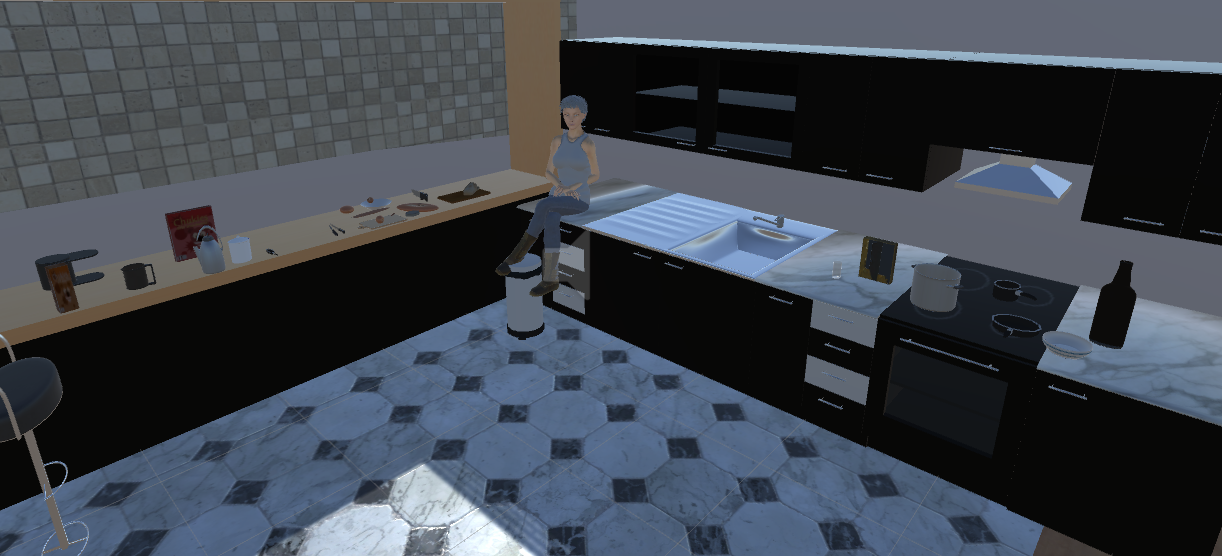
\includegraphics[width=0.7\linewidth]{images/kitchen}
		\caption{Kitchen environment}
		\label{fig:kitchen}
	\end{figure}
	
	In order to create a living representation of the world, all materials were split to different categories. Tools - knifes, spoons, and all cooking related. Ingredients - vegetables, meals, coffee, sugar, salt. Sources - Cups, Saucepans, Plates, Stoves. Their functionality follows same as in real world. \\
	This approach was chosen not only for simple process logic. It can be used for a teaching purposes, to show patients how to act with different kinds of objects. \\
	
	$ Seazing\ all\ activities\ were\ removed.\ They require\ carefull\ logic\ approach. $
	
	In terms of the tools, they exist independently and EvKa watches over their state during entire process. They have to be at particular area, can not be dropped and never must face to a person direction. Using a motion tracker those warning can be re-enabled. Currently, she just watch if it was dropped or not, and returns to origin location. \\
	
	Ingredients are the same as a tools, excepted that they can change their state during cooking process. They can be washed, cut, fried, frozen. Currently only few of those straits implemented. Depending on complexity of the tasks, these may be enabled. To unfreeze meat, time calculates based on conditions around, vegetable can be washed after collision with water source. \\
	
	Sources are content for ingredients. Those are final stages for making food. After combining all ingredients, it calculates or sets time for cooking. After, Evka just monitors conditions and provides reminder in the cooking process. \\
	
	Those are basic tasks which person expect to do around kitchen. \\
	
	\textbf{	Calculating temperature around} \\
	Considering that it happens in Virtual World, there is a possibility to simulate certain events. Same way, using some school physics formula, it allows to calculate cooking time, based on room conditions~\eqref{eqn:eqlabel}. 
	

	\begin{flalign} \label{eqn:eqlabel}
		TT & = 100 * ((v * 8.33 * 453.59237) * (((5 / 9) * (ET - 32)) - ((5 / 9) * (ST - 32))) / (eg * 0.238845896628 * eff)) / 60; & \\
		Where, & \\			
		TT & = Time\ to\ Temperature & \\
		v & = Volume\ (Gallons) & \\
		ET & = End\ Temperature\ (Fahrenheit) & \\
		ST & = Start\ Temperature\ (Fahrenheit) & \\
		eff & = Efficiency & \\
		eg & = Energy \\
	\end{flalign}



	
	RTVoive capable of using Windows Mac voice and MarryTTS - adaptive served voice. Allows change sharpens, type and speed of voice acting, if necessary. All lines are stored in one particular C\# script. Which means can be easily retranslated or rewriten. 	
	
	\subsubsection{Knife and cutting tools}
	Figure~\ref{fig:knife_spoon} represents implemented examples of cutting tools. Their main property for this game is to collide with food type objects and change their states. For example, by colliding knife with onion, it will become "cut onion", which is an ingredient for the receipt. \\
		\begin{figure}[H]
			\centering
			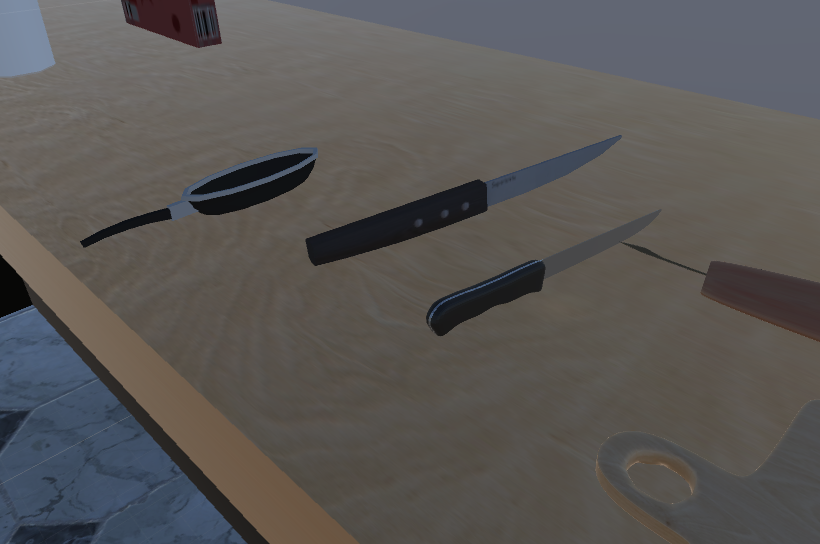
\includegraphics[width=0.5\linewidth]{images/knife_spoon}
			\caption{Knifes}
			\label{fig:knife_spoon}
		\end{figure}
	One of implemented properties, is that knife never should leave working area. By drooping knife on the floor, will make it as possible source of danger. For now, Eva will inform it, and place it back where belongs. In addition, knife never should leave coocking table. It will be inappropriate if knife will end up somewhere out of kitchen. Eva will simply lose from control view. However, it is not a problem insight the game, but may be dangerous in real life. Moreover,it is restricted to collide knife with leaving being like person or Virtual Avatar. If with Evka, it will end up with simple warning, person may injure himself. This action will completely drop Eva's mood and stop everything what's been happening around. \\
	In order to approach task management problem, such as knife can not be used as spoon, knife hasn't been provided with Mixing tag. In other words, if Eva notice that person mixes a coffee with knife, instead of spoon, she will not consider coffee complete. This idea should give a person understanding that different task must be managed with certain tool. \\
	\subsubsection{Meat and Vegetables}
	Ingredients, shown of Figure~\ref{fig:food} does not have anything particular except the tag and different states. Currently, the most stable and appropriate way to change states of Vegetables is to apply certain script to each type. \\
		\begin{figure}[H]
			\centering
			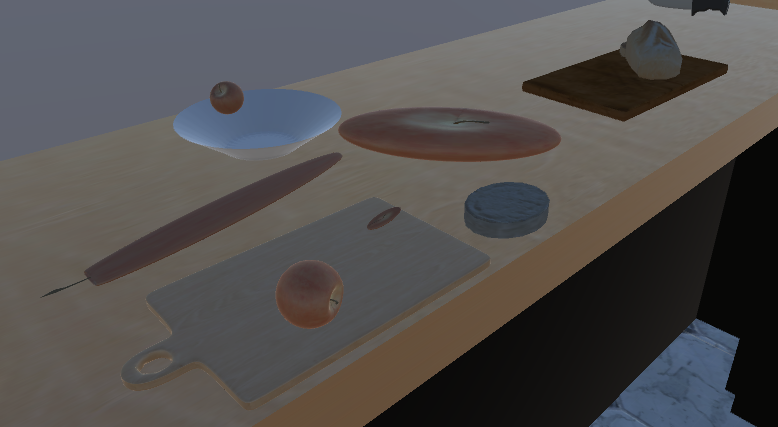
\includegraphics[width=0.5\linewidth]{images/food}
			\caption{Knifes}
			\label{fig:food}
		\end{figure}
	In order to universalise entire approach with vegetables, it will be wise to create separate independent structure, in which states of the product will simply change in one particular order. Idea was left for future work. \\
	\subsubsection{Cooking Pans}
	Figure~\ref{fig:pans} represents implemented pans in the game. They serve some sort of container who stores objects which were collided with it. After, Eva can compare them and give certain output, and start timer. In addition, pans also can be source of danger. Spilling the content will lead to the loos of ingridients and starts process again. However, it is not equaly dangerous as a knife, and accidents can happen in working area, Eva will consider it, but situations still affects her mood.
		\begin{figure}[H]
			\centering
			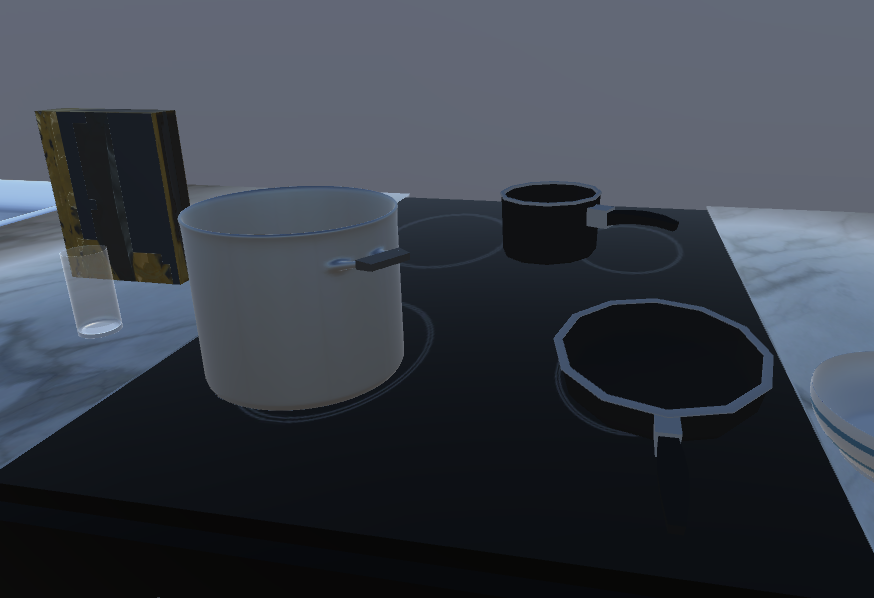
\includegraphics[width=0.5\linewidth]{images/pans}
			\caption{Cooking Pans}
			\label{fig:pans}
		\end{figure}
	
	\subsubsection{Evka}
	In order to attract person attention and keep his mind occupied, Evka received a human body, which acts as a support\\adviser around kitchen. Her abilities extend at entire area, however as a person she located at place, which is  view, but does not affect process around. She also acts as Audio Source, as basic interaction abilities like talking, greeting and idle sitting. Her skills as a person can be extended, depending how living she must be, right now she capable only to track persons view and call for his attention, he gets distracted. \\
	\begin{figure}[H]
		\centering
		\begin{subfigure}{0.4\textwidth}
			\centering
			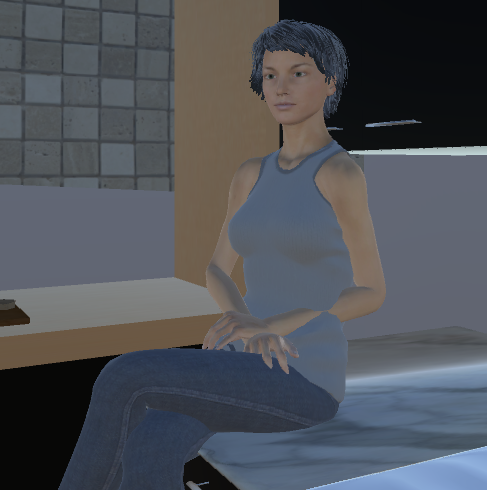
\includegraphics[width=1\linewidth]{images/Evka_sit_1}
			\caption{Evka's idle sitting}
		\end{subfigure}
		\begin{subfigure}{0.4\textwidth}
			\centering
			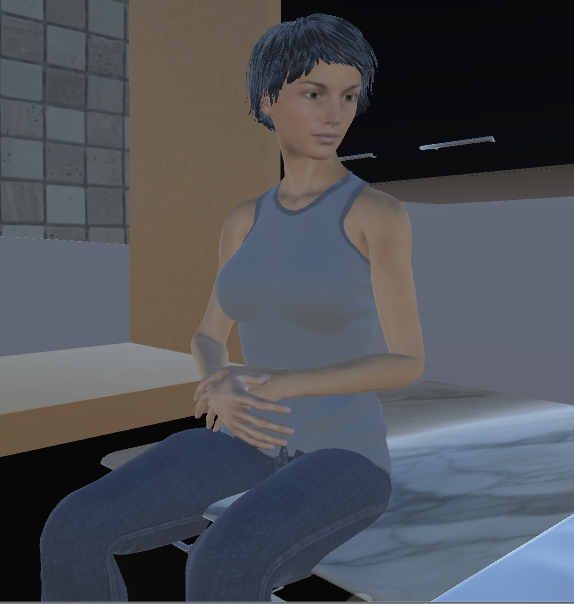
\includegraphics[width=0.96\linewidth]{images/Evka_sit_2}
			\caption{Evka's idle talking}
		\end{subfigure}		
		\caption{Evka}
		\label{fig:evkasit1}
	\end{figure}
	
	
	Currently, her voice is product of inbuilt Windows or Mac Voices, it maybe not emotional, but contains general understanding of the tasks. This approach will make sure that patients are still occupied with cooking process. If not - she will remind him or her. \\	
	
	Eva has a pre-sets of animation, which avatar expected to be performedm on Figure~\ref{fig:animat}. Process of installing them has no difference from any other unity projects. One of the Evka's abilities is to point toward objects around. This function is used in case if person gets lost around. She is able to remind patient to grab something, or use it toward vegetables or saucepan. Waiving was used for simple greeting at the beginning, however it may become useful if person gets lost around Virtual Reality. Moreover, Eva's body used as Audio Source to recreate illusion of real person. \\
	\begin{figure}[H]
		\centering
		\begin{subfigure}{0.2\textwidth}
			\centering
			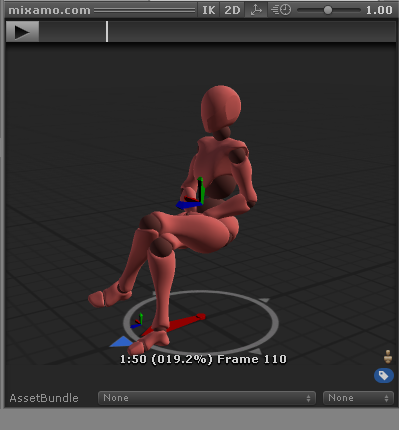
\includegraphics[width=1\linewidth]{images/sit}
			\caption{Idle sitting}
		\end{subfigure}
		\begin{subfigure}{0.2\textwidth}
			\centering
			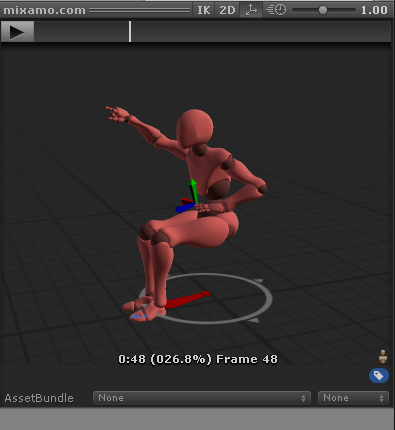
\includegraphics[width=0.96\linewidth]{images/sit_point}
			\caption{Pointing toward object}
		\end{subfigure}		
		\begin{subfigure}{0.2\textwidth}
			\centering
			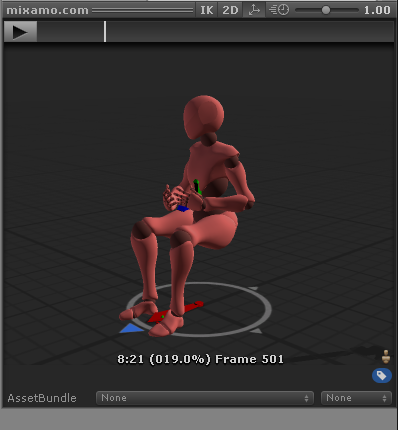
\includegraphics[width=0.96\linewidth]{images/sit_talk}
			\caption{Idle Talking}
		\end{subfigure}
		\begin{subfigure}{0.2\textwidth}
			\centering
			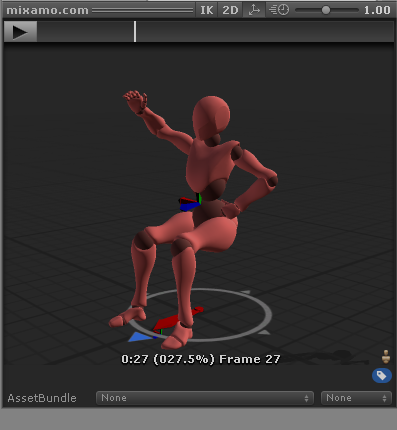
\includegraphics[width=0.96\linewidth]{images/sit_wave}
			\caption{Greeting}
		\end{subfigure}				
		\caption{Supported Animation}
		\label{fig:animat}
	\end{figure}
	
	\subsection{Instruction and Guidance}
	
	In order to demonstrate the process of easy creation of the new item in the kitchen, following instruction will be provided.\\
	
	First you have an area. Drop any item which you want to add to surrounding. Manipulate with sizes and add one of pre existed tags, $\left(\ or\ create\ a\ new\ one\ if\ necessary,\ it\ may\ require\ longer\ process\  \right) . $ Figure~\ref{fig:add_object} shows added Onion. In order to apply basic manipulation rules, it most be added to the list of objects around, as shown in the code. \\
	
	\begin{figure}[H]
		\centering
		\begin{subfigure}{0.45\textwidth}
			\centering
			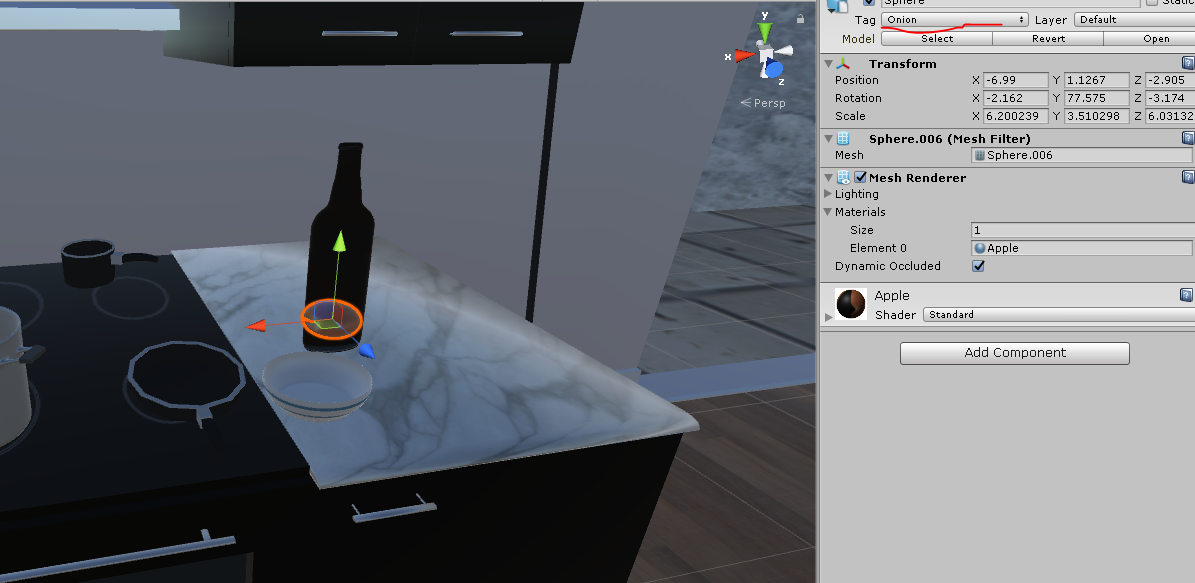
\includegraphics[width=1\linewidth]{images/add_onion}
			\caption{Adding onion}
		\end{subfigure}
		\begin{subfigure}{0.45\textwidth}
			\centering
			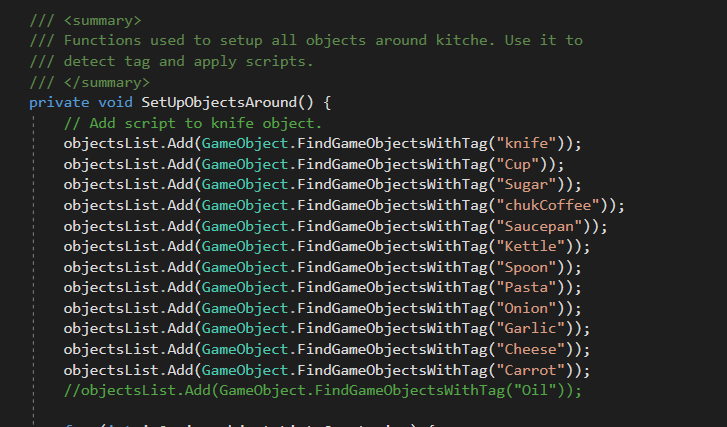
\includegraphics[width=0.85\linewidth]{images/add_onion_code}
			\caption{Code for onion}
		\end{subfigure}		
		\caption{Evka}
		\label{fig:add_object}
	\end{figure}
	
	Program will automatically apply basic transform scripts. Take for example we want to add fraying pan an extra tool. After adding it to a world and applying Saucepan's tag, it will be able to store content, which called ingredients for cooking, as all necessary scripts will be applied. Figure~\ref{fig:add_franpan} shows game before and after run. \\
	
	\begin{figure}[H]
		\centering
		\begin{subfigure}{0.45\textwidth}
			\centering
			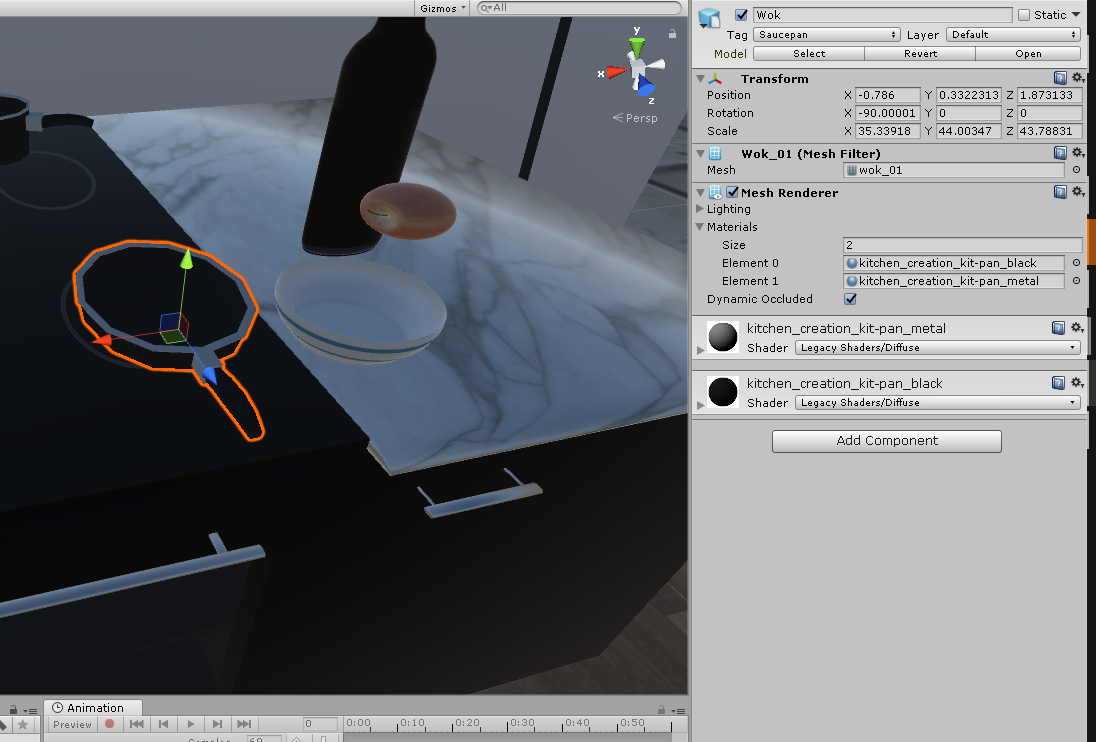
\includegraphics[width=1\linewidth]{images/franpan}
			\caption{Evka's idle sitting}
		\end{subfigure}
		\begin{subfigure}{0.45\textwidth}
			\centering
			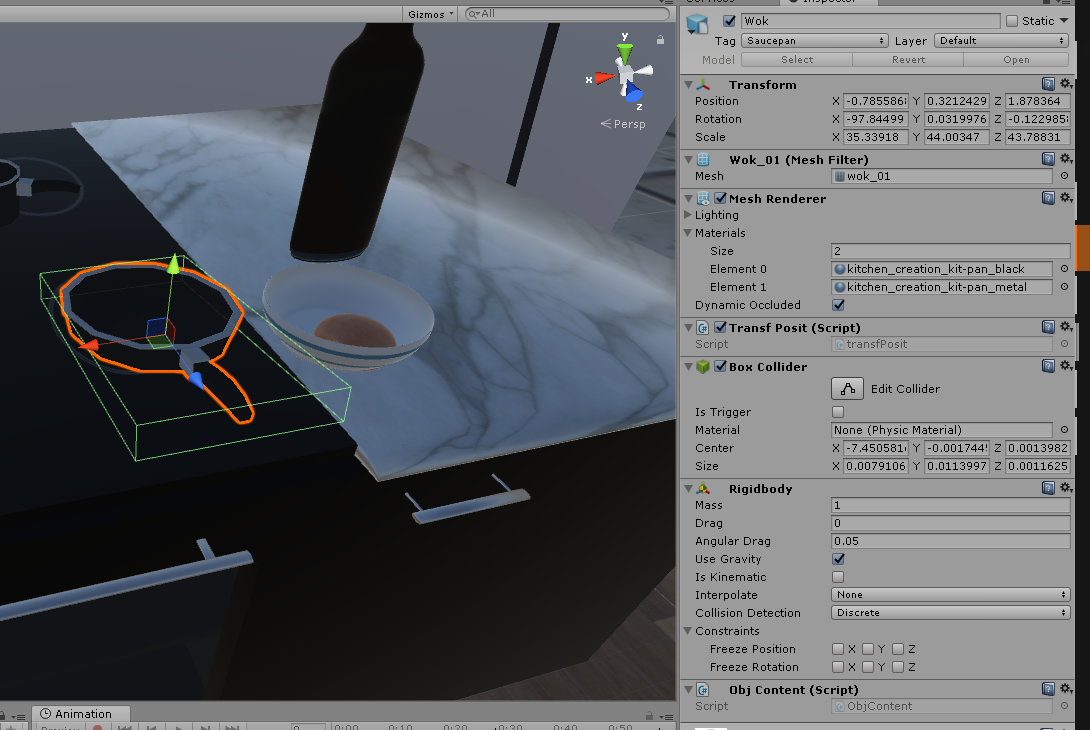
\includegraphics[width=1\linewidth]{images/franpan_script}
			\caption{Evka's idle talking}
		\end{subfigure}		
		\caption{Evka}
		\label{fig:add_franpan}
	\end{figure}
	
	Second, create a recipe. Better if it will be stored somewhere accessible. Script named $receipts$ contains all current staff possible to cook. As an example, lets create a receipt for stir-fry mince with onion cooked on the olive oil. We assume that pasta already ready and it's not part of receipt. $ \left(such\ complex\ receipts\ will\ require\ more\ manipulation.  \right) $ Create and Array List with strings, which contains oil, onion, mince, mixed. Last word will mean that content must be stirring with any object which can do it, like spoon. Time for cooking may be calculated automatically with formulas and room conditions, or can be parsed and presented, it will be showed later. \\
	
	\lstset{style=sharpc}
	\begin{lstlisting}
	using System.Collections.Generic;
	/// <summary>
	/// Contains information about all receipts which used in cooking
	/// </summary>
	internal class receiptsList {    
		public List<string> receiptCoffe { get { 
				return new List<string> { "water", "coffee", "sugar" ,"mixed"}; } }
				
		public List<string> receiptPasta { get { 
				return new List<string> { "Boiled", "pasta" }; } }
		
		// Newly added receipt		
		public List<string> receiptPastaInNavy { get { 
				return new List<string> { "onion", "oil", "mince", "mixed" }; } }
	}
	\end{lstlisting}
	
	Sooner or later it will be noticed that mince does not actually exist in the world either. However, this is not a difficult process to perform. Drop any item which you want and add tag mince, same one you used in receipt and perform same manipulation as with onion. Later it will be shown how to add different states of mince. As soon as collision will be performed with pan, object will be considered to be added to container. \\
	
	The last step is to perform actual cooking process. In the main script, following lines must be added on top of other processes. How this scrips perform work in writen in API, but long story short, it must set what to cook by adding receipt, where cooking must be performed, and what Eva must say then cooking started or there some problems with ingridients. Those lines are optional, it used in case if something else must be performed after cook. Timer accepts condition of the room, plate etc. User is free to set own time.
	
	\lstset{style=sharpc}
	\begin{lstlisting}
	stuffToMake.Add(new CookProcc {
		Ingridients = recLists.receiptPastaInNavy,
		Contents = GetParticularObjects("Saucepan"),
		SuccessString = "Good Work. Now you have to wait until they ready. I will inform you then time run out",
		MissingString = "You missing a ",	// Says then something missing from list
		ExtraString = "Why did you add ",	// Says if something extra added
		Timer = equations.CalculateBoilingTime(2, 100, 26, 2000, 300)
	});
	\end{lstlisting}
	By default EvKa's dialogues will remainder about remaining time or other actions required, they also can be modified from this call or through timer set up. Basically this is a process of basic cooking. All other processes followed with other instructions. \ldots
	
	If cooking process requires other manipulation with object like changing a state from solid to messed, it can be performed through modefying a loop with paricular code \ldots \ldots If process requires harder manipulation, then appropriate scripts must be created and added in the same loop as Game Component. 
	
	\subsection{Worlds Logic.}
	In order to understand processes which occurs around, it is better to view them separately. As it's been already discussed, it consist of 3 types of tool. Every tool type monitored by their own independent rules, which can not be broken. This designed to keep user in certain boundaries then he is not in the process of cooking something particular. This approach also allow perform some multitasking operations. All of them are united by one unique cooking process. The example approach, which was mentioned above, showed how logic is united to perform one particular task. However, EvKa can leave focus on user reaction, and focus on the states of objects around. If their condition may cause any danger - certain response will be called.
	
	Response of EvKa's reaction depends on her level of the mood. This approach makes her feel a bit as living being, and as soon as her patience runs out, she will call for assistance from supervisor.
	\subsubsection{Strips algorithm}
	\subsubsection{Temperature \& Time Calculation}
	\subsubsection{Dialogues System}
	
\section{Conclusion}
	\subsection{Results}
	\begin{enumerate}
		\item What was achieved? - Environment designed, algorithm adaptive, dialogues created.
		\item Portability. - Extract pachage, prefab..
		\item Augemented reality research
		\item What has become with Evka
	\end{enumerate}
	As a result of two months research and development, design wend through several modifications. At the end, resulting product came to VI, which able track state of the objects around, give certain feedback and serve as virtual assistant. Logic behind is easily adaptable and can be reused for other tasks around kitchen. This will totally depend on clients desire and persons abilities. \\
	
	However, this is not  guaranty total independence, but it will a first step to something greater in the future. \\
	\subsection{Ideas for future}
	
	\textbf{ ADD AS FUTURE WORK. At final product, there will be no reasons adding controllers to persons hand, instead cameras or Kinect tool will track objects around and their movements.  Players must have augmented reality set in order to see an avatar, if necessary and all other warning, visual and audio.\\}
	
\section{Acknowledgements}	
	Virtual environment was created using several different assets form Unity Assets Store. THose credits belongs to: 
	\begin{enumerate}
		\item Kitchen Creation Kit - Adding environment tools
		\item Kitchen Asset - Creating kitchen environment
		\item MORPH3D - Evka's body and Clothes based on model of (Cyria).
		\item RTVoice - Adds Voice to Avatar.
	\end{enumerate}
	
	In addition, I want to thank VRES for providing this opportunity, along side with SEF. Great thanks Dr Ross Brown, for guiding through entire research last two months. \\	
	
%===================================================%
%													%
%============Bibliography and refferencing==========%
%												    %
%===================================================%
\newpage
\begin{flushleft}
\bibliographystyle{referencing/IEEEtran}
\bibliography{referencing/referenceList}

\end{flushleft}

\end{document}
